\documentclass[12pt]{article}
\usepackage{a4wide, amsfonts, epsfig,bbding,phonetic}

\begin{document}
\begin{center}
{\bf EMAT10001 Lecture 16.}\\[1cm]{} Conor Houghton 2014-2-16
\end{center}
\subsection*{Preface} 
These are outline notes for lecture 16. As usual there is a bounty of
between 20p and \pounds 2 for errors, you can tell me at the end of a
lecture or email me at \texttt{conor.houghton{@}bristol.ac.uk}.

\subsection*{Introduction}

This is a lecture about partial differentiation and the gradient
vector.

\subsection*{Partial differentiation}

So, when we differentiate a function, we are working out its rate of change:
\begin{equation}
\frac{df}{dt}=\lim_{h\rightarrow 0}\frac{f(t+h)-f(t)}{h}
\end{equation}
That is, it tells us how much $f(t)$ is increasing as $t$ increases,
at exactly the point $t$. Now, functions can depend on more than one
variable, so we could have $f(x,y)$ for example. Now, at it's
simplest, the partial derivative calculates how the function changes as one
of the variables changes.
\begin{equation}
\frac{\partial f}{\partial x}=\lim_{h\rightarrow 0}\frac{f(x+h,y)-f(x,y)}{h}
\end{equation}
and
\begin{equation}
\frac{\partial f}{\partial y}=\lim_{h\rightarrow 0}\frac{f(x,y+h)-f(x,y)}{h}
\end{equation}
Note the partial sign, $\partial$, instead of the $d$, to denote
partial differentiation. Make sure you write these two characters
differently!

In practice, this means that when taking the partial derivative with
respect to $x$ you act as if $y$ is a constant and visa versa. Hence, if
\begin{equation}
f(x,y)=xy^2+x^2+y
\end{equation}
then
\begin{equation}
\frac{\partial f}{\partial x}=y^2+2x
\end{equation}
and 
\begin{equation}
\frac{\partial f}{\partial y}=2xy+1
\end{equation}

\subsection*{The gradient vector and the directional derivative}

Often $x$ and $y$ aren't the only directions you are interested in and
what you want is the \textsl{directional derivative}, the derivative in some other direction. The most convenient way to describe a direction mathematically is with a unit vector
\begin{equation}
\mathbf{n}=(n_1,n_2)
\end{equation}
with $\sqrt{n_1^2+n_2^2}=1$. Here, I am using the bold notation for
vectors, this is the most common notation although in school
mathematics an arrow over the letter is common. One potentially
confusing thing is that in hand-written mathematics the bold is
indicated with an underline, so $\underline{n}$ in hand writing to the
same as $\mathbf{n}$ in print, just like \lq{}a\rq{} in print is the
same as \lq{}\vara\rq{} in handwritting. Anyway, the idea is that a
vector has direction and length, but a unit vector is always one long,
so it is used to define direction. 

Now, the directional derivative, written $\nabla_{\textbf{n}}$ is a measure of how much $f$ changes in the direction $\mathbf{n}$. We could write $\textbf{x}=(x,y)$ and
\begin{equation}
\nabla_{\textbf{n}}f(\mathbf{x})=\lim_{h\rightarrow 0}\frac{f(\textbf{x}+h\textbf{n})-f(\textbf{x})}{h}
\end{equation}
or, equivalently
\begin{equation}
\nabla_{\textbf{n}}f(x,y)=\lim_{h\rightarrow 0}\frac{f(x+hn_1,y+hn_2)-f(x,y)}{h}
\end{equation}
Luckily there is an easy formula for this
\begin{equation}
\nabla_{\textbf{n}}f(\mathbf{x})=\mathbf{\nabla}f\cdot\mathbf{n}
\end{equation}
where $\mathbf{\nabla}f$ is the \textsl{gradient} of $f(x,y)$
\begin{equation}
\mathbf{\nabla}f=\left(\frac{\partial f}{\partial x},\frac{\partial f}{\partial y}\right)
\end{equation}
Thus, the gradient of $f(x,y)$ is a vector made out of the partial
derivatives. It is sometimes written as grad$f$ so
\begin{equation}
\mbox{grad}f=\mathbf{\nabla}f
\end{equation}

The formula for the directional derivative says it is the
dot product of the gradient with the direction vector. To remind you,
if $\mathbf{a}=(a_1,a_2)$ and $\mathbf{b}=(b_1,b_2)$ are two vectors then their dot product is
\begin{equation}
\mathbf{a}\cdot\mathbf{b}=a_1b_1+a_2b_2=|\mathbf{a}||\mathbf{b}|\cos{\theta}
\end{equation}
where $\theta$ is the angle between $\mathbf{a}$ and $\mathbf{b}$. If
$\mathbf{n}$ is a unit vector then $\mathbf{a}\cdot\mathbf{n}$ is a
\textsl{projection} of $\mathbf{a}$ into the direction $\mathbf{n}$;
it shows how much of $\mathbf{a}$ lies in the direction $\mathbf{n}$. In this way we can think of the gradient desribing how $f$ is changing and the directional derivative as saying how much of that change is in the direction.

\begin{figure}
\begin{center}
\setlength{\unitlength}{4144sp}%
\begingroup\makeatletter\ifx\SetFigFont\undefined%
\gdef\SetFigFont#1#2#3#4#5{%
  \reset@font\fontsize{#1}{#2pt}%
  \fontfamily{#3}\fontseries{#4}\fontshape{#5}%
  \selectfont}%
\fi\endgroup%
\begin{picture}(3627,1404)(1339,-4153)
\put(1351,-3661){\vector( 1, 0){900}}
\put(1351,-3661){\vector( 2, 1){1800}}
\multiput(1351,-3661)(114.28571,0.00000){32}{\line( 1, 0){ 57.143}}
\multiput(3151,-2761)(0.00000,-120.00000){8}{\line( 0,-1){ 60.000}}
\multiput(1801,-4111)(-128.57143,0.00000){4}{\line(-1, 0){ 64.286}}
\put(1351,-4111){\vector(-1, 0){0}}
\multiput(2701,-4111)(128.57143,0.00000){4}{\line( 1, 0){ 64.286}}
\put(3151,-4111){\vector( 1, 0){0}}
\put(1801,-3286){\makebox(0,0)[lb]{\smash{{\SetFigFont{12}{14.4}{\rmdefault}{\mddefault}{\updefault}{$\mathbf{a}$}%
}}}}
\put(1576,-3886){\makebox(0,0)[lb]{\smash{{\SetFigFont{12}{14.4}{\rmdefault}{\mddefault}{\updefault}{$\mathbf{n}$}%
}}}}
\put(4951,-3436){\makebox(0,0)[lb]{\smash{{\SetFigFont{12}{14.4}{\rmdefault}{\mddefault}{\updefault}{$\mathbf{n}$-direction}%
}}}}
\put(2026,-4111){\makebox(0,0)[lb]{\smash{{\SetFigFont{12}{14.4}{\rmdefault}{\mddefault}{\updefault}{$\mathbf{a}\cdot\mathbf{n}$}%
}}}}
\end{picture}%
\end{center}
\caption{The dot-product: $\mathbf{a}\cdot\mathbf{n}$ gives the length of the perpendicular projection of $\mathbf{a}$ onto the direction indicated by the unit vector $\mathbf{n}$.}
\end{figure}

\begin{figure}
\begin{center}
% GNUPLOT: LaTeX picture with Postscript
\begingroup
  \makeatletter
  \providecommand\color[2][]{%
    \GenericError{(gnuplot) \space\space\space\@spaces}{%
      Package color not loaded in conjunction with
      terminal option `colourtext'%
    }{See the gnuplot documentation for explanation.%
    }{Either use 'blacktext' in gnuplot or load the package
      color.sty in LaTeX.}%
    \renewcommand\color[2][]{}%
  }%
  \providecommand\includegraphics[2][]{%
    \GenericError{(gnuplot) \space\space\space\@spaces}{%
      Package graphicx or graphics not loaded%
    }{See the gnuplot documentation for explanation.%
    }{The gnuplot epslatex terminal needs graphicx.sty or graphics.sty.}%
    \renewcommand\includegraphics[2][]{}%
  }%
  \providecommand\rotatebox[2]{#2}%
  \@ifundefined{ifGPcolor}{%
    \newif\ifGPcolor
    \GPcolorfalse
  }{}%
  \@ifundefined{ifGPblacktext}{%
    \newif\ifGPblacktext
    \GPblacktexttrue
  }{}%
  % define a \g@addto@macro without @ in the name:
  \let\gplgaddtomacro\g@addto@macro
  % define empty templates for all commands taking text:
  \gdef\gplbacktext{}%
  \gdef\gplfronttext{}%
  \makeatother
  \ifGPblacktext
    % no textcolor at all
    \def\colorrgb#1{}%
    \def\colorgray#1{}%
  \else
    % gray or color?
    \ifGPcolor
      \def\colorrgb#1{\color[rgb]{#1}}%
      \def\colorgray#1{\color[gray]{#1}}%
      \expandafter\def\csname LTw\endcsname{\color{white}}%
      \expandafter\def\csname LTb\endcsname{\color{black}}%
      \expandafter\def\csname LTa\endcsname{\color{black}}%
      \expandafter\def\csname LT0\endcsname{\color[rgb]{1,0,0}}%
      \expandafter\def\csname LT1\endcsname{\color[rgb]{0,1,0}}%
      \expandafter\def\csname LT2\endcsname{\color[rgb]{0,0,1}}%
      \expandafter\def\csname LT3\endcsname{\color[rgb]{1,0,1}}%
      \expandafter\def\csname LT4\endcsname{\color[rgb]{0,1,1}}%
      \expandafter\def\csname LT5\endcsname{\color[rgb]{1,1,0}}%
      \expandafter\def\csname LT6\endcsname{\color[rgb]{0,0,0}}%
      \expandafter\def\csname LT7\endcsname{\color[rgb]{1,0.3,0}}%
      \expandafter\def\csname LT8\endcsname{\color[rgb]{0.5,0.5,0.5}}%
    \else
      % gray
      \def\colorrgb#1{\color{black}}%
      \def\colorgray#1{\color[gray]{#1}}%
      \expandafter\def\csname LTw\endcsname{\color{white}}%
      \expandafter\def\csname LTb\endcsname{\color{black}}%
      \expandafter\def\csname LTa\endcsname{\color{black}}%
      \expandafter\def\csname LT0\endcsname{\color{black}}%
      \expandafter\def\csname LT1\endcsname{\color{black}}%
      \expandafter\def\csname LT2\endcsname{\color{black}}%
      \expandafter\def\csname LT3\endcsname{\color{black}}%
      \expandafter\def\csname LT4\endcsname{\color{black}}%
      \expandafter\def\csname LT5\endcsname{\color{black}}%
      \expandafter\def\csname LT6\endcsname{\color{black}}%
      \expandafter\def\csname LT7\endcsname{\color{black}}%
      \expandafter\def\csname LT8\endcsname{\color{black}}%
    \fi
  \fi
  \setlength{\unitlength}{0.0500bp}%
  \begin{picture}(5040.00,3528.00)%
    \gplgaddtomacro\gplbacktext{%
      \csname LTb\endcsname%
      \put(699,986){\makebox(0,0){\strut{}-10}}%
      \put(1242,892){\makebox(0,0){\strut{}-5}}%
      \put(1785,797){\makebox(0,0){\strut{} 0}}%
      \put(2327,703){\makebox(0,0){\strut{} 5}}%
      \put(2869,608){\makebox(0,0){\strut{} 10}}%
      \put(3092,670){\makebox(0,0){\strut{}-10}}%
      \put(3406,834){\makebox(0,0){\strut{}-5}}%
      \put(3719,998){\makebox(0,0){\strut{} 0}}%
      \put(4032,1161){\makebox(0,0){\strut{} 5}}%
      \put(4345,1325){\makebox(0,0){\strut{} 10}}%
      \put(683,1522){\makebox(0,0)[r]{\strut{} 0}}%
      \put(683,1738){\makebox(0,0)[r]{\strut{} 50}}%
      \put(683,1953){\makebox(0,0)[r]{\strut{} 100}}%
      \put(683,2169){\makebox(0,0)[r]{\strut{} 150}}%
      \put(683,2386){\makebox(0,0)[r]{\strut{} 200}}%
    }%
    \gplgaddtomacro\gplfronttext{%
      \put(3376,2804){\makebox(0,0)[r]{\strut{}$x^2+y^2$}}%
    }%
    \gplbacktext
    \put(0,0){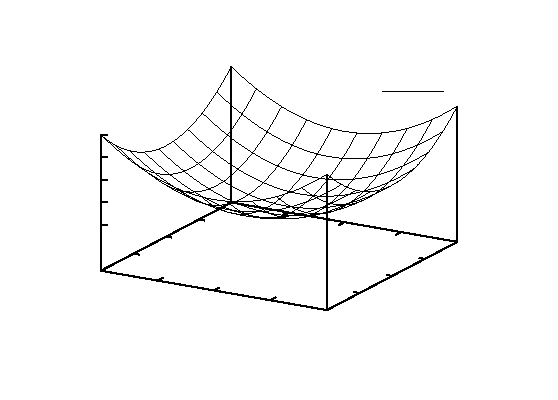
\includegraphics{x2y2}}%
    \gplfronttext
  \end{picture}%
\endgroup

\end{center}
\caption{The function $x^2+y^2$ is shaped like a bowl.}
\end{figure}

Lets do a quick example, consider 
\begin{equation}
f(x,y)=x^2+y^2
\end{equation}
and say you want the derivative in the direction
\begin{equation}
\mathbf{n}=\frac{1}{\sqrt{2}}(1,-1)
\end{equation}
at the point $(2,2)$. Well
\begin{equation}
\mathbf{\nabla}f=\left(2x,2y\right)
\end{equation}
so at $(2,2)$ we have 
\begin{equation}
\mathbf{\nabla}f|_{(2,2)}=\left(4,4\right)
\end{equation}
and hence the directional derivative is 
\begin{equation}
(1,-1)\cdot(4,4)=4-4=0
\end{equation}
This makes sense because if you think of the symmetry of function it
doesn't change if you go around. 

\subsection*{The direction of change}

Now, lets look at the directional derivative again
\begin{equation}
\nabla_{\mathbf{n}}f(x,y)=\mathbf{\nabla}f\cdot \mathbf{n}=|\mathbf{\nabla}f|\cos{\theta}
\end{equation}
 where, again, $\theta$ is the angle between $\mathbf{\nabla}f$ and
 $\mathbf{n}$. Clearly this is biggest when $\theta=0$, that is, when
 $\mathbf{n}$ is in the same direction as $\mathbf{\nabla}f$. Thus,
 $\mathbf{\nabla}f$ points in the direction $f(x,y)$ is changing in
 fastest, the direction with the largest directional derivative. In
 the bowl example above, for example, $\mathbf{\nabla}f=(2x,2y)$, that
 is, it always points straight outwards, straight up the side of the
 bowl.

Without going into details here, gradients are important in some areas
of computer science because of \textsl{gradient descent}. This is an
approach to minimizing a function of lots of variables. In machine
learning, for example, this function might be an error function,
expressing how an estimate differs from the thing it estimates. In
gradient descent the gradient vector is used to decide how to reduce
the error by, as it were, heading straight down the gradient hill. In
fact, the story is a bit more complicated, because of the hazard
presented by thin valleys in the error landscape, a slightly different
method is used, called \textsl{conjugate gradient}.

\subsection*{Other differential operators}
The gradient is one of three common differential operators. Another
common operator is the \textsl{divergence}; the gradient acts on
scalar functions to give a vector, the divergence is the other way
around, it acts on vectors to give a scalar function. Say $\mathbf{f}$
is a vector function, in two-dimensions it might be 
\begin{equation}
\mathbf{f}(x,y)=(f_1(x,y),f_2(x,y))
\end{equation}
The divergence of $\mathbf{f}$ is then
\begin{equation}
\mbox{div}\mathbf{f}=\mathbf{\nabla}\cdot\mathbf{f}=\frac{\partial f_1}{\partial x}+\frac{\partial f_2}{\partial y}
\end{equation}

Here is a rough interpretation. Imagine the vector field is the
velocity of a gas, in some places the vectors are getting shorted
because it's somewhere the gas is slowing down, in others they are
getting longer because the gas is speeding up. In some places the gas
is spreading out, so the directions are changing. The divergence at a
point will measure whether the density of the gas at the point is going up or
down. It measures whether the velocity vector field is changing in such a way as would cause the gas to accumulate or its opposite. 

\end{document}

